\documentclass[
    11pt,
    a4paper
]{article}

% =========================================================
% IDIOMA, CODIFICACIÓN Y TIPOGRAFÍA
% =========================================================

\usepackage[utf8]{inputenc}
\usepackage[T1]{fontenc}
\usepackage{csquotes}
\usepackage[french]{babel}
\usepackage{lmodern}
\usepackage{microtype}

% =========================================================
% GEOMETRÍA DE LA PÁGINA
% =========================================================

\usepackage[
    top=2.5cm,
    bottom=2.5cm,
    left=2.8cm,
    right=2.8cm
]{geometry}

% =========================================================
% MATEMÁTICAS
% =========================================================

\usepackage{amsmath}
\usepackage{amssymb}
\usepackage{amsfonts}
\usepackage{mathtools}
\usepackage{bm}

% =========================================================
% UNIDADES Y NOTACIÓN CIENTÍFICA
% =========================================================

\usepackage{siunitx}

\sisetup{
    output-decimal-marker={,},
    separate-uncertainty=true,
    per-mode=symbol
}

% =========================================================
% FIGURAS
% =========================================================

\usepackage{graphicx}
\usepackage{float}
\usepackage{subcaption}
\usepackage{placeins}

% Carpeta en la que se almacenarán las figuras
\graphicspath{{figures/}}

% =========================================================
% TABLAS
% =========================================================

\usepackage{booktabs}
\usepackage{tabularx}
\usepackage{array}
\usepackage{multirow}
\usepackage{longtable}

% =========================================================
% COLORES
% =========================================================

\usepackage{xcolor}

\definecolor{linkcolor}{RGB}{0,70,140}
\definecolor{citecolor}{RGB}{0,100,70}
\definecolor{urlcolor}{RGB}{120,40,120}

% =========================================================
% CÓDIGO
% =========================================================

\usepackage{listings}

\lstdefinestyle{pythonstyle}{
    language=Python,
    basicstyle=\ttfamily\small,
    numbers=left,
    numberstyle=\tiny,
    stepnumber=1,
    numbersep=8pt,
    frame=single,
    breaklines=true,
    showstringspaces=false,
    tabsize=4,
    captionpos=b
}

\lstset{style=pythonstyle}

% =========================================================
% HIPERVÍNCULOS Y REFERENCIAS CRUZADAS
% =========================================================

\usepackage[
    colorlinks=true,
    linkcolor=linkcolor,
    citecolor=citecolor,
    urlcolor=urlcolor,
    bookmarksopen=true,
    bookmarksnumbered=true
]{hyperref}

\usepackage[nameinlink, noabbrev]{cleveref}

% Nombres utilizados por cleveref
\crefname{equation}{équation}{équations}
\Crefname{equation}{Équation}{Équations}

\crefname{figure}{figure}{figures}
\Crefname{figure}{Figure}{Figures}

\crefname{table}{tableau}{tableaux}
\Crefname{table}{Tableau}{Tableaux}

\crefname{section}{section}{sections}
\Crefname{section}{Section}{Sections}

\crefname{subsection}{sous-section}{sous-sections}
\Crefname{subsection}{Sous-section}{Sous-sections}

% =========================================================
% ENCABEZADOS Y PIES DE PÁGINA
% =========================================================

\usepackage{fancyhdr}

\pagestyle{fancy}
\fancyhf{}

\fancyhead[L]{Convergence numérique de la force de coupe (Étape 0)}
\fancyhead[R]{\thepage}
\setlength{\headheight}{14.2pt}

\renewcommand{\headrulewidth}{0.4pt}
\renewcommand{\footrulewidth}{0pt}

% =========================================================
% FORMATO DE TÍTULOS
% =========================================================

\usepackage{titlesec}

\titleformat{\section}
    {\Large\bfseries}
    {\thesection.}
    {0.5em}
    {}

\titleformat{\subsection}
    {\large\bfseries}
    {\thesubsection.}
    {0.5em}
    {}

% =========================================================
% ESPACIADO
% =========================================================

\usepackage{setspace}

\setstretch{1.15}
\setlength{\parindent}{0pt}
\setlength{\parskip}{0.6em}

% =========================================================
% BIBLIOGRAFÍA
% =========================================================

\usepackage[
    backend=biber,
    style=numeric,
    sorting=none
]{biblatex}

\addbibresource{references.bib}

% =========================================================
% COMANDOS PERSONALIZADOS
% =========================================================

\newcommand{\ap}{a_p}
\newcommand{\fz}{f_z}
\newcommand{\kf}{k_f}
\newcommand{\Ac}{A_c}
\newcommand{\Fref}{F_{\mathrm{ref}}}
\newcommand{\dxlsize}{\Delta_{\mathrm{dxl}}}
\newcommand{\RMS}{\operatorname{RMS}}

% =========================================================
% INFORMACIÓN DEL DOCUMENTO
% =========================================================

\title{
    \textbf{Vérification de la convergence numérique de la force de coupe simulée en fonction de la taille de dexel (Étape 0)}
}

\author{
    Enrique Mireles
}

\date{\today}

% =========================================================
% INICIO DEL DOCUMENTO
% =========================================================

\begin{document}

\maketitle

\begin{abstract}

Ce document présente la procédure théorique et numérique utilisée pour vérifier que la
force de coupe simulée par un modèle géométrique discrétisé (représentation en dexels)
converge vers une force de référence analytique, calculée à partir d'un modèle
mécaniciste de coupe, lorsque la taille de discrétisation \(\dxlsize\) diminue. Quatre
estimateurs d'erreur relative sont définis (biais de la moyenne, erreur de crête, étendue
et écart-type) et utilisés pour identifier, sur un plan d'expériences (DOE) balayant
\(\dxlsize\), la taille de dexel la plus grossière garantissant une convergence numérique
suffisante avant l'extraction des indicateurs de détection du chatter (SPRT/MaxEnt,
SSQ-STFT, Green Integral) dans les étapes suivantes.

\end{abstract}

\tableofcontents

\newpage

\section{Introduction}
\label{sec-introduction}

Dans les simulations étudiées, la géométrie de la matière enlevée est représentée par une
discrétisation en dexels, dont la taille \(\dxlsize\) fixe la résolution spatiale du
modèle géométrique : plus \(\dxlsize\) est faible, plus la discrétisation est fine et plus
le coût de calcul est élevé.

Avant d'utiliser la force de coupe simulée pour en extraire un indicateur de détection du
chatter, il est nécessaire de s'assurer que cette force ne soit pas polluée par des
artefacts numériques liés à la discrétisation géométrique. Cette étape correspond à une
étude de convergence de maillage au sens classique du calcul numérique
% TODO: cite Roache (1998), Verification and Validation in Computational Science and Engineering
: on compare la force simulée à une force de référence analytique indépendante du
maillage, pour un balayage de valeurs de \(\dxlsize\), et on identifie la valeur la plus
grossière pour laquelle l'écart reste inférieur à un seuil de tolérance fixé (\SI{10}{\percent}).
Ce seuil constitue une convention personnelle, pour laquelle un écart de cet ordre sur les
efforts de coupe est jugé acceptable et exploitable en pratique.

Cette étude est un préalable indispensable : si la force simulée présente une variance ou
un biais d'origine purement numérique, les indicateurs statistiques utilisés en aval pour
détecter le chatter (basés sur la variance, l'entropie spectrale ou l'énergie du signal de
force) ne pourront pas distinguer ce bruit numérique d'une véritable instabilité
dynamique.

\section{Modèle mécaniciste de force de référence}
\label{sec-modele_force_ref}

La force de référence \(\Fref\) est calculée à partir d'un modèle mécaniciste linéarisé de
la force de coupe, cas limite du modèle de Kienzle--Victor
% TODO: cite Kienzle-Victor (1952) et sa generalisation au fraisage (Altintas)
lorsque l'exposant de taille de copeau \(m_c \to 0\), c'est-à-dire lorsque la pression
spécifique de coupe \(\kf\) est traitée comme constante :

\begin{equation}
    \Ac = \ap \, \fz,
    \label{eq-section_coupe}
\end{equation}

\begin{equation}
    \Fref = \kf \, \Ac,
    \label{eq-force_ref}
\end{equation}

où \(\ap\) [mm] est la profondeur axiale de coupe, \(\fz\) [mm/tour] l'avance par tour
(cas d'un tournage à une seule arête de coupe) et \(\kf\) [N/mm\(^2\)] la pression
spécifique de coupe. L'{}\cref{eq-section_coupe} donne la section de copeau non déformé
\(\Ac\) [mm\(^2\)].

Les grandeurs cinématiques associées à la discrétisation temporelle sont

\begin{equation}
    \Delta t = \frac{60}{\Omega \, N_{\mathrm{rev}}},
    \label{eq-dt}
\end{equation}

\begin{equation}
    V_f = \Omega \, \fz \times 10^{-3},
    \label{eq-vf}
\end{equation}

où \(\Omega\) [tr/min] est la vitesse de rotation et \(N_{\mathrm{rev}}\) le nombre de pas
de temps par tour. L'{}\cref{eq-dt} fixe la résolution angulaire de la simulation
(\(360^\circ/N_{\mathrm{rev}}\) par pas de temps), indépendante de \(\dxlsize\) mais dont la
finesse doit être vérifiée séparément pour ne pas contaminer l'étude de convergence
spatiale.

Le cas simulé correspond à une opération de tournage, et non de fraisage : l'outil ne
comporte qu'une seule arête de coupe, de sorte que \(N_t=1\) est ici une caractéristique
exacte de l'opération -- et non une approximation -- et n'a donc pas à apparaître
explicitement dans \cref{eq-vf}. Plus précisément, il s'agit d'un cas simplifié de
tournage à un seul degré de liberté (1DDL), à profondeur de passe \(\ap\) constante, pour
lequel la dynamique structurelle a été désactivée (simulation purement cinématique). Le
modèle dynamique complet associé à ce cas est présenté dans une section antérieure de la
thèse ; la présente étude de convergence en prépare le terrain en validant, en amont, la
fiabilité numérique de la force simulée qui alimentera ce modèle. La géométrie de la pièce
est un cylindre -- et non un cône -- de rayon extérieur constant.

\section{Estimateurs d'erreur de convergence}
\label{sec-estimateurs_erreur}

Soit \(F(t)\) la composante de force simulée extraite du signal \texttt{res\_R\_p},
restreinte à une fenêtre temporelle \([t_{\mathrm{start}}, t_{\mathrm{end}}]\) excluant le
régime transitoire d'engagement de l'outil. Quatre estimateurs d'erreur relative,
exprimés en pourcentage de \(\Fref\), sont calculés pour chaque cas du DOE :

\begin{equation}
    e_{\mathrm{biais}} = \frac{\left| \bar{F} - \Fref \right|}{\Fref} \times 100,
    \qquad
    \bar{F} = \frac{1}{N}\sum_{i=1}^{N} F(t_i),
    \label{eq-err_mean}
\end{equation}

\begin{equation}
    e_{\text{crête}} = \frac{\max\big(|F_{\max}-\Fref|,\; |F_{\min}-\Fref|\big)}{\Fref} \times 100,
    \label{eq-err_peak}
\end{equation}

\begin{equation}
    e_{\text{étendue}} = \frac{|F_{\max} - F_{\min}|}{\Fref} \times 100,
    \label{eq-err_range}
\end{equation}

\begin{equation}
    e_{\text{écart-type}} = \frac{\sigma_F}{\Fref} \times 100,
    \qquad
    \sigma_F = \sqrt{\frac{1}{N}\sum_{i=1}^{N} \big(F(t_i)-\bar{F}\big)^2},
    \label{eq-err_std}
\end{equation}

où \(F_{\max}\) et \(F_{\min}\) sont les valeurs extrémales de \(F(t)\) sur la fenêtre
considérée.

L'{}\cref{eq-err_mean} quantifie le biais systématique de l'estimateur par rapport à la
valeur théorique. L'{}\cref{eq-err_peak} borne l'erreur au pire cas ponctuel, pertinente car
la force de coupe est intrinsèquement périodique. L'{}\cref{eq-err_range} est sensible aux
artefacts de discrétisation géométrique de type \emph{staircase}, caractéristiques des
représentations par dexels/voxels lorsque la taille de cellule est grossière.
L'{}\cref{eq-err_std} est l'estimateur le plus directement lié à la variance d'origine
numérique : à convergence (\(\dxlsize \to 0\), en l'absence de vibration physique réelle),
\(\sigma_F\) devrait tendre vers une valeur faible et stable, toute fluctuation résiduelle
étant alors un artefact purement numérique.

\section{Procédure numérique}
\label{sec-procedure}

Le balayage de \(\dxlsize\) utilisé pour cette étude comporte douze cas, issus du fichier
\texttt{doe\_\allowbreak results.h5} du plan d'expériences
\texttt{0\_Cinematique/\allowbreak DOE\_Dexels\_Cinematique}, couvrant la plage
\(\dxlsize \in [4\times10^{-5},\ 2,56\times10^{-3}]\)~m, sans critère de répartition
particulier entre ces valeurs.

Pour chaque cas \texttt{case\_XXX} de ce fichier :

\begin{enumerate}
    \item lecture du signal de force \texttt{res\_R\_p} et de l'attribut \(\dxlsize\)
        associé au cas (fonction \texttt{read\_force\_values});
    \item calcul de la moyenne temporelle et de l'erreur de biais,
        \cref{eq-err_mean} (\texttt{compute\_\allowbreak force\_stats});
    \item calcul, sur la fenêtre \([t_{\mathrm{start}}, t_{\mathrm{end}}]\), des erreurs de
        crête, d'étendue et d'écart-type, \cref{eq-err_peak,eq-err_range,eq-err_std}
        (\texttt{compute\_\allowbreak force\_\allowbreak error\_\allowbreak window},
        \texttt{compute\_\allowbreak force\_\allowbreak spread\_\allowbreak error\_\allowbreak window},
        \texttt{compute\_\allowbreak force\_\allowbreak std\_\allowbreak error\_\allowbreak window});
    \item écriture des quatre estimateurs, ainsi que des constantes utilisées
        (\(\Fref\), \(\Ac\), \(V_f\), \(\Delta t\)), comme attributs et jeux de données du
        groupe HDF5 du cas.
\end{enumerate}

Une fois tous les cas traités, les quatre estimateurs sont tracés en fonction de
\(\dxlsize\) sous forme de diagramme en barres groupées (fonction
\texttt{fig3\_error\_summary}), avec une ligne de seuil à \SI{10}{\percent} et la mise en
évidence de la taille de dexel retenue pour les étapes suivantes du pipeline.

\begin{figure}[H]
    \centering
    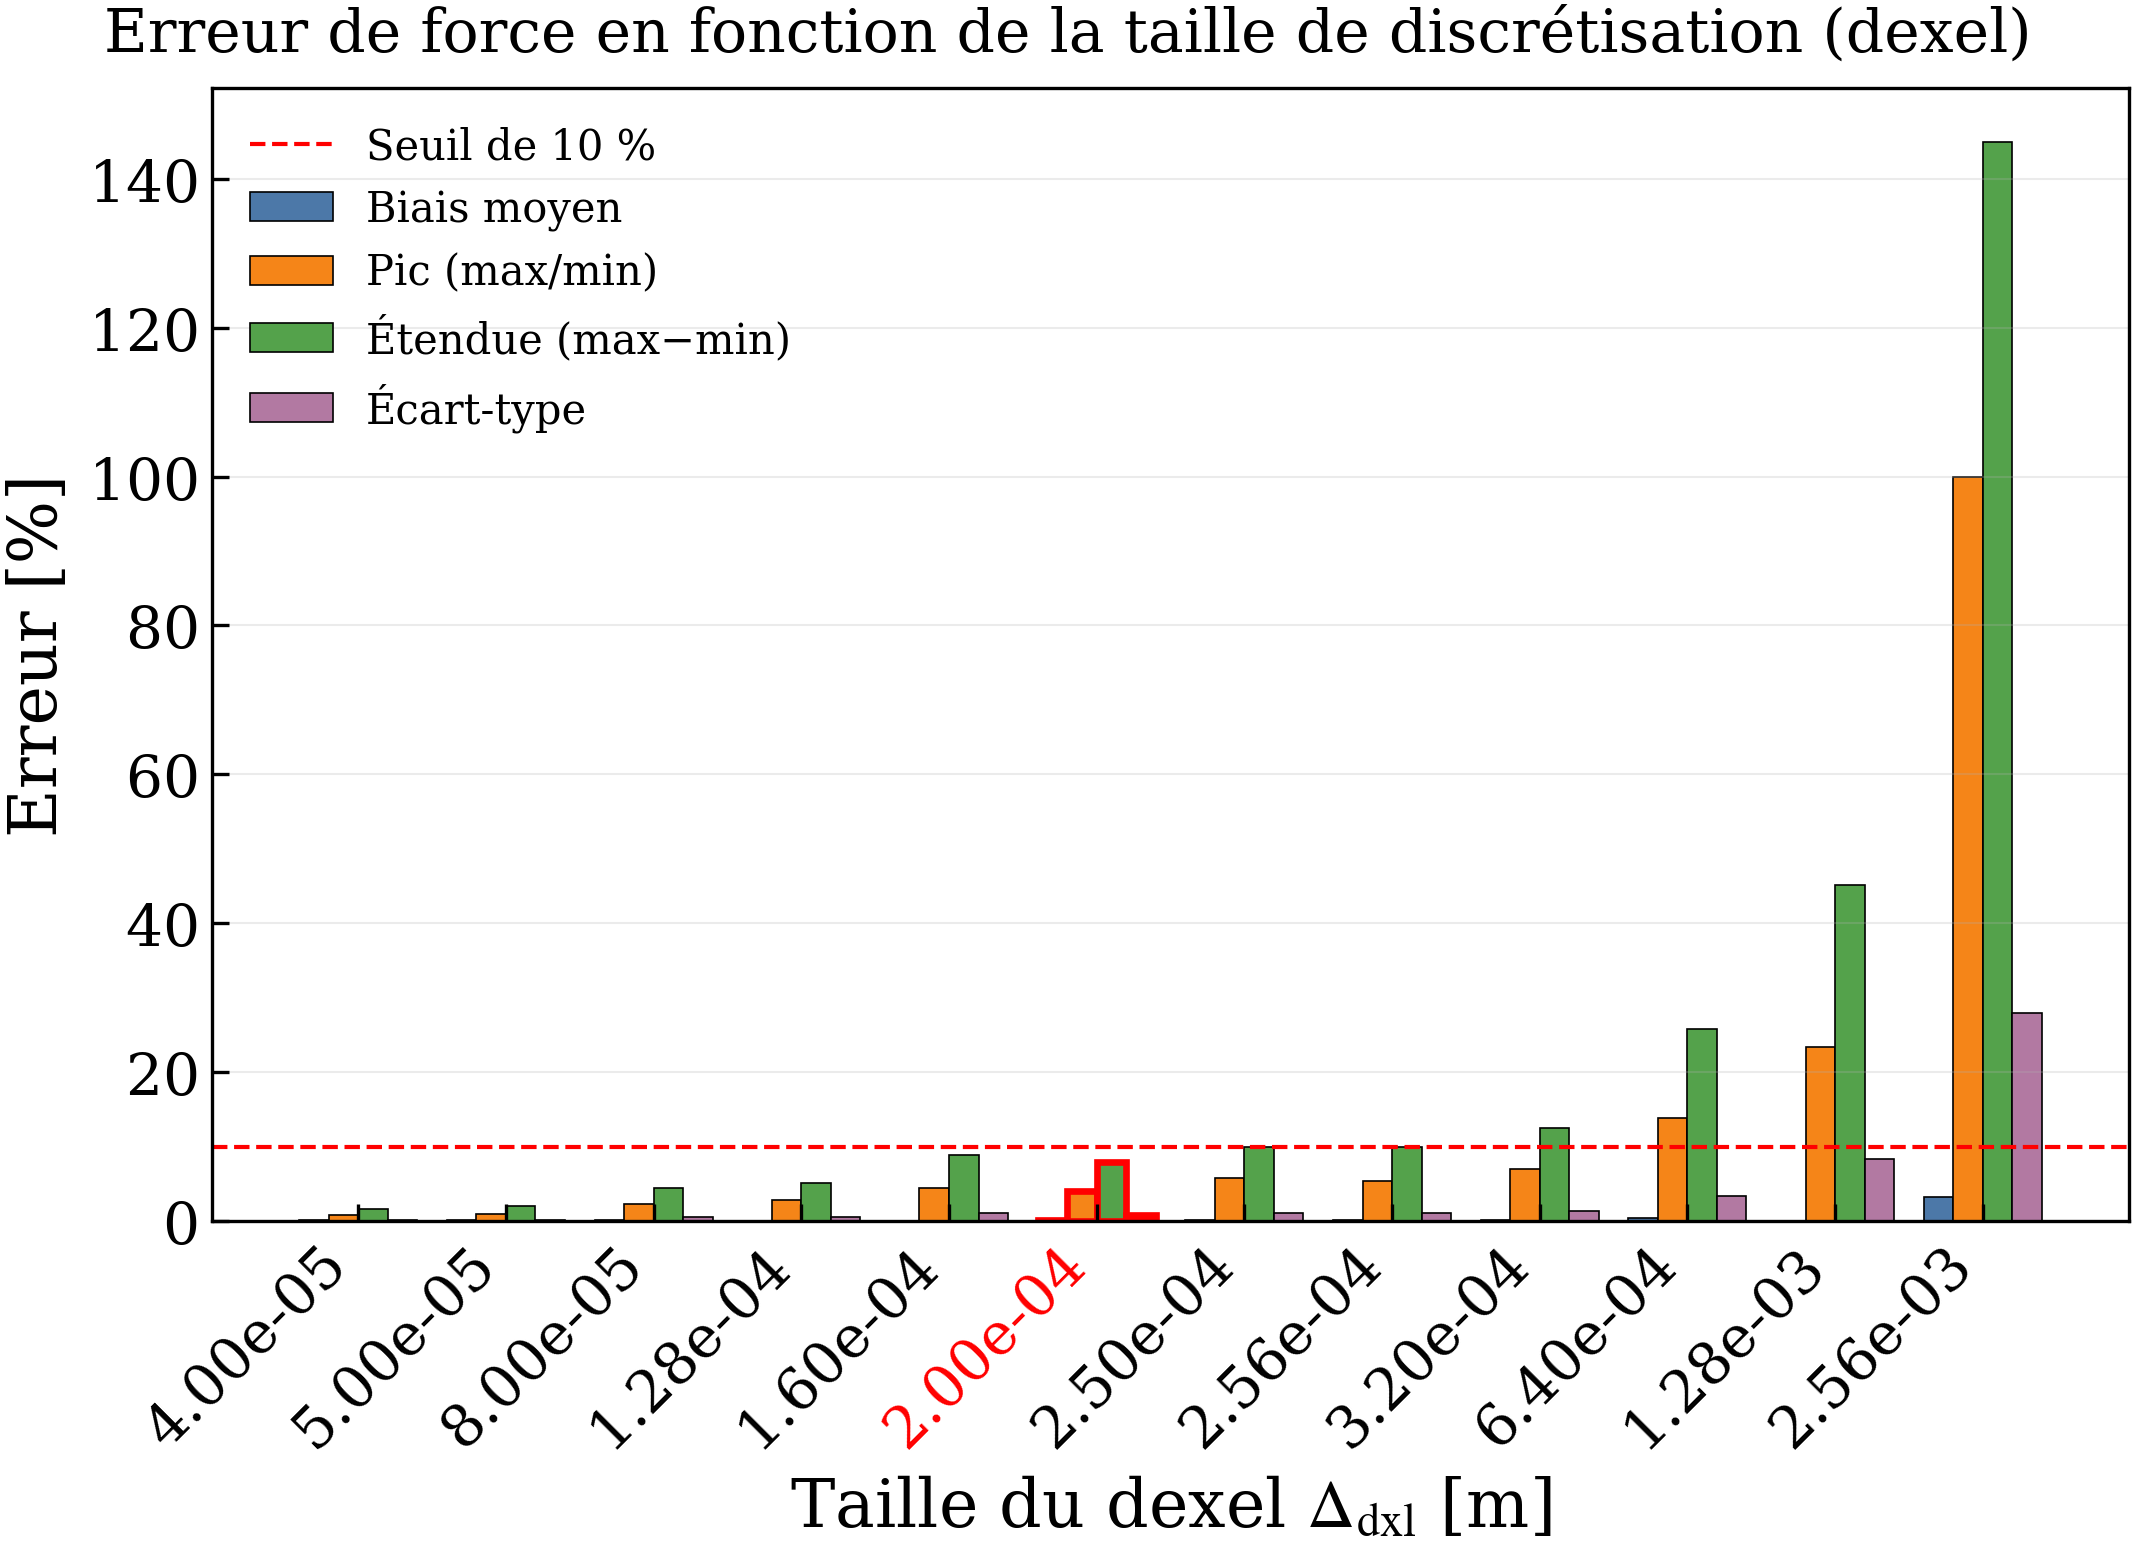
\includegraphics[width=\linewidth]{fig3_error_summary}
    \caption{Erreur relative de la force simulée par rapport à \(\Fref\), pour les quatre
    estimateurs définis en \cref{sec-estimateurs_erreur}, en fonction de la taille de
    dexel \(\dxlsize\). La ligne pointillée indique le seuil de tolérance de
    \SI{10}{\percent}.}
    \label{fig-err_summary}
\end{figure}

On observe sur la \cref{fig-err_summary} que l'erreur croît avec la taille de dexel
\(\dxlsize\), sans qu'il s'agisse d'une relation linéaire. Caractériser précisément la
relation entre \(\dxlsize\) et l'erreur ne fait pas l'objet de ce travail, mais deux
tendances qualitatives se dégagent : en doublant \(\dxlsize\), l'erreur augmente de façon
nettement plus que proportionnelle, alors qu'en divisant \(\dxlsize\) par deux
(raffinement), l'amélioration de l'erreur, bien que présente, reste limitée. Cette allure
évoque une croissance de type exponentiel, sans qu'aucune régression n'ait été réalisée
pour confirmer cette forme -- ce point resterait à vérifier quantitativement. Au-delà de
\(\dxlsize = 3,2\times10^{-4}\)~m, l'erreur augmente nettement plus rapidement, en
particulier pour les estimateurs de crête \(e_{\text{crête}}\) et d'étendue
\(e_{\text{étendue}}\) (\cref{eq-err_peak,eq-err_range}). De façon générale, les quatre
estimateurs suivent une évolution qualitativement similaire avec \(\dxlsize\) -- seul leur
ordre de grandeur diffère.

La valeur retenue pour les étapes suivantes du pipeline est \(\dxlsize = 2\times10^{-4}\)~m
(soit \(20\times10^{-5}\)~m), mise en évidence en rouge sur la \cref{fig-err_summary}. Ce
choix résulte d'un compromis recherché entre finesse de discrétisation et coût de calcul :
la tolérance de \SI{10}{\percent} fixe le niveau de finesse jugé suffisant, et
\(\dxlsize = 2\times10^{-4}\)~m est la valeur la plus grossière -- donc la moins coûteuse en
temps de calcul -- pour laquelle les quatre estimateurs d'erreur restent simultanément sous
ce seuil, le critère le plus contraignant étant celui de l'étendue \(e_{\text{étendue}}\)
(\cref{eq-err_range}). Cette valeur constitue également un point de départ raisonnable pour
explorer, dans les étapes suivantes, des tailles de dexel aussi bien plus fines que plus
grossières sans risquer un coût de calcul excessif.

% TODO: si les temps de calcul par cas (wall_time_s.txt, un par sous-dossier de
% 0_Cinematique/DOE_Dexels_Cinematique/) sont exploites, ajouter ici une figure/tableau
% du cout de calcul en fonction de dxl_size pour etayer quantitativement ce compromis
% finesse/cout -- a confirmer avec l'utilisateur avant de la generer.

\section{Hypothèses et conditions de validité}
\label{sec-hypotheses}

\begin{itemize}
    \item Le modèle de force \cref{eq-force_ref} est linéarisé (\(\kf\) constant) : il ne
        capture pas l'effet de taille (\emph{size effect}) du modèle de Kienzle complet,
        et n'est valable ici que comme référence déterministe pour l'étude de
        convergence, pas comme prédiction précise de la force physique réelle.
    \item \(\Fref\) est une valeur statique/cinématique pure, sans retard régénératif ni
        dynamique de structure. La comparaison à cette référence n'est donc valide que si
        la simulation de l'{}\hyperref[sec-procedure]{Étape 0} correspond à une coupe sans
        vibration structurelle -- toute oscillation de \(F(t)\) est alors attribuable à la
        discrétisation, non à un phénomène physique.
    \item La fenêtre temporelle exclut le régime transitoire d'engagement
        (\(t \geq t_{\mathrm{start}}\)), supposé non représentatif du régime établi.
    \item La discrétisation temporelle (\(N_{\mathrm{rev}}\), \cref{eq-dt}) est supposée
        suffisamment fine pour que l'erreur observée provienne uniquement de
        \(\dxlsize\); ceci devrait être vérifié séparément par une étude de convergence
        équivalente sur \(N_{\mathrm{rev}}\).
\end{itemize}

\section{Conclusion}
\label{sec-conclusion}

Cette vérification de convergence constitue l'Étape 0 du pipeline : elle établit,
quantitativement et avec un critère d'acceptation explicite, la taille de dexel la plus
grossière pour laquelle la force simulée peut être considérée comme numériquement
convergée, à savoir \(\dxlsize = 2\times10^{-4}\)~m (\cref{fig-err_summary}). Cette
condition remplie, le signal de force peut être utilisé de façon fiable
comme entrée des indicateurs de détection du chatter (SPRT/MaxEnt, entropie spectrale
SSQ-STFT, Green Integral) étudiés dans les étapes suivantes, sans risque de confondre
artefact numérique et instabilité dynamique réelle.

% \printbibliography

\end{document}
